
\subsection{Analisi delle risposte dei sistemi del secondo ordine}
\label{sec:analisi_secondo_ordine}
Si considera il caso di un sistema del secondo ordine con due poli reali e
distinti, ha la seguente funzione di trasferimento
$$
W(s) =\frac{K_B}{(1+s\tau_1)(1+s\tau_2)}
$$
con $\tau_1 > \tau_2$,
\begin{figure}[h]
 \centering
 \begin{tikzpicture}
  \begin{axis}[
   width=0.6\linewidth,
   height=0.3\linewidth,
   axis lines = middle,
   xtick={-2,-1,0},
   ytick={0},
   xlabel={\Re},
   ylabel={\Im},
   xmax=0.3,xmin=-2.5,ymin=-0.3,ymax=1,
   xticklabels={$p_2$,$p_1$,0},
   ]
\filldraw(-1,0) circle (2pt)
         (-2,0) circle (2pt);
  \end{axis}
 \end{tikzpicture}
\end{figure}
dunque $p_1$ è il polo dominante.

Si analizza la risposta all'impulso
$$
W(t) = \Lap^{-1}[W(s)] =
\frac{K_B}{\tau_1\tau_2}\Lap^{-1}\left[\frac{R_1}{s+\frac{1}{\tau_1}} +
\frac{R_2}{s+\frac{1}{\tau_2}}\right]
$$
L'eccesso poli zeri è pari a due, dunque la sommatoria dei residui deve essere
pari a zero. $R_1 = \frac{\tau_1\tau_2}{\tau_1-\tau_2} \rightarrow R_2 = -R_1 =
\frac{\tau_1\tau_2}{\tau_2-\tau_1}$.
$$
W(t) =
K_B\frac{1}{\tau_1-\tau_2}\left(e^{-\frac{t}{\tau_1}}-e^{-\frac{t}{\tau_2}}
\right)\delta_{-1}(t)
$$
Si mostra l'andamento normalizzato rispetto al guadagno statico e le costanti
di tempo.
\begin{figure}[h]
 \centering
 \begin{tikzpicture}
  \begin{axis}[
   width = 0.6\linewidth,
   axis lines = middle,
   ylabel={$(\tau_2-\tau_1)\frac{W(t)}{K_B}$},
   xlabel={$t$},
   xtick={0,0.33,1},
   xticklabels={,$\tau_2$,$\tau_1$},
   ytick={-1,0,1},
   %yticklabels={},
   x tick label style={yshift=1.5em},
   xlabel style={at={(ticklabel* cs:1)},anchor=north},
   ylabel style={at={(ticklabel* cs:1)},anchor= east},
   ymax=1.3,
   ymin=-1.1,
   ]
   \addplot[domain=0:3,samples=60]{exp{-x}};
   \addplot[domain=0:1,dashed]{1-x};
   \addplot[domain=0:3,samples=60]{-exp(-3*x)};
   \addplot[domain=0:0.333,dashed]{3*x-1};
   \addplot[domain=0:3,color = red,samples=100,
   line width =0.2mm]{exp(-x)-exp(-3*x)};
   %\addplot[]{x};
  \end{axis}
 \end{tikzpicture}
\end{figure}
La funzione raggiunge un picco e tende poi a decrescere al valore
dell'esponenziale
con la costante di tempo maggiore.

\subsubsection{Risposta al gradino}
Si vuole calcolare la risposta al gradino, antitrasformata della funzione di
trasferimento moltiplicata la trasformata del gradino
$\left(\frac{1}{s}\right)$.
$$\begin{aligned}
W_{-1}(t) &= \Lap^{-1}\left[ \frac{W(s)}{s} \right] =
\Lap^{-1}\left[\frac{R_0}{s} + \frac{R_1}{s+\frac{1}{\tau_1}} + \frac{R_2}
{s+\frac{1}{\tau_2}}
\right]\frac{K_B}{\tau_1\tau_2} = \\
&=K_B\left( 1 -
\frac{\tau_1}{\tau_1-\tau_2}e^{-\frac{t}{\tau_1}} +
\frac{\tau_2}{\tau_1-\tau_2}e^{-\frac{t}{\tau_2}}\right)\delta_{-1}(t)
\end{aligned}$$
L'eccesso poli-zeri è ancora pari a due ma l'ingresso è un gradino, ricordando
la tabella \ref{tab.:stato-uscita} si vede che la derivata prima e seconda
sono nulle nell'origine.

%definizione tau per i due grafici a seguire
\def\tOne{1.6}
\def\tTwo{0.6}
\def\dt{(\tOne-\tTwo)}
\begin{figure}[h]
 \centering
 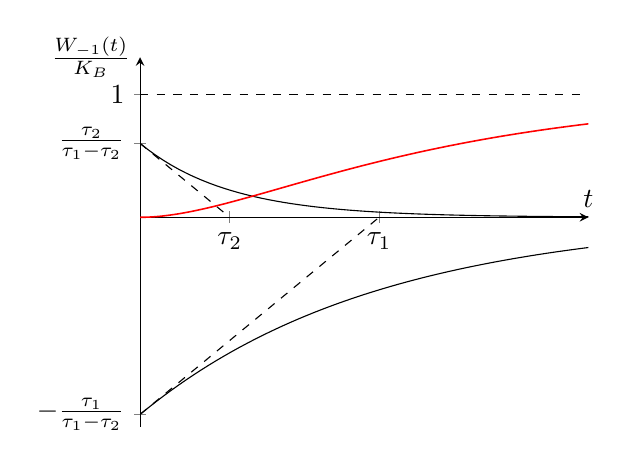
\begin{tikzpicture}
 %\def\tOne{1.6}
 %\def\tTwo{0.6}
 %\def\dt{(\tOne-\tTwo)}
  \begin{axis}[
   width = 0.6\linewidth,
   axis lines = middle,
   ylabel={$\frac{W_{-1}(t)}{K_B}$},
   xlabel={$t$},
   xtick={0,\tTwo,\tOne},
   xticklabels={,$\tau_2$,$\tau_1$},
   ytick={-\tOne/\dt,0,\tTwo/\dt,1},
yticklabels={$-\frac{\tau_1}{\tau_1-\tau_2}$,0,$\frac{\tau_2}{\tau_1-\tau_2}$,1}
,
   %x tick label style={yshift=1.5em},
   xlabel style={at={(ticklabel* cs:1)},anchor=south},
   ylabel style={at={(ticklabel* cs:1)},anchor= east},
   ymax=1.3,
   ymin=-\tOne/\dt-0.1,
   xmin=0,
   xmax=3,
   ]
   \addplot[domain=0:3,samples=60]{-(\tOne/\dt)*exp(-x/\tOne)};
   \draw[dashed](0,{\tTwo/\dt})--(\tTwo,0);
   \draw[dashed](0,{-\tOne/\dt})--(\tOne,0);
   \draw[dashed] (0,1)--(3,1);
   \addplot[domain=0:3,samples=60]{(\tTwo/\dt)*exp(-x/\tTwo)};
   %\addplot[domain=0:0.333]{3*x-1};
   \addplot[domain=0:3,color = red,samples=100,
   line width =0.2mm]{1-(\tOne/\dt)*exp(-x/\tOne)+(\tTwo/\dt)*exp(-x/\tTwo)};
   %\addplot[]{x};
  \end{axis}
 \end{tikzpicture}
 \caption{Risposta al gradino sistema secondo ordine}
 \label{fig.:gradino_secondo_ordine}
\end{figure}
In questo caso con $\tau_1 = \tOne$ e $\tau_2 = \tTwo$ si vede molto la
prevalenza della funzione con costante più
lenta sulla risposta, l'uscita tende asintoticamente ad uno.
Nel caso particolare in cui $\tau_1 = \tau_2$ ossia due poli coincidenti
$$
W_{-1}(t) = K_B \left( 1 - e^{-\frac{t}{\tau}} -
\frac{t}{\tau}e^{-\frac{t}{\tau}}
\right)\delta_{-1}(t)
$$
L'andamento sarà comunque simile al caso generale.

\newpage
\subsection{Analisi risposta funzione con uno zero}
La funzione in analisi del secondo ordine ha anche uno zero al numeratore
$$
W(s) =
\frac{K_B\left(1+s_{\tau_z}\right)}{\left(1+s_{\tau_1}\right)
\left(1+s_{\tau_2}\right)} \qquad \tau_1>\tau_2
$$
A seconda della posizione dello zero rispetto ai poli si avranno soluzioni
differenti.
Si analizza il caso in cui $\tau_z = 0$ ossia lo zero si trova sull'asse reale
a $-\infty$.
$$
W(s) = K_B \frac{1}{(1+s\tau_1)(1+s\tau_2)} + K_B
\frac{s\tau_z}{(1+s\tau_1)(1+s\tau_2)}
$$
La risposta impulsiva sarà data da due contributi nel tempo, il primo identico
a quanto calcolato alla sezione \ref{sec:analisi_secondo_ordine}; il secondo
termine invece differisce dal primo per $s\tau$, $\tau$ è un fattore di scala,
la $s$ invece indica la derivata nel tempo, dunque il secondo termine è
pari alla derivata del primo contributo.
La risposta al gradino sarà dunque:
$$
W_{-1}(t) = K_B \left(1 -
\frac{\tau_1-\tau_z}{\tau_1-\tau_2}e^{-\frac{t}{\tau_1}} +
\frac{\tau_2-\tau_z}{\tau_1-\tau_2}e^{-\frac{t}{\tau_2}}
\right)\delta_{-1}(t)
$$
Prendendo riferimento dalla figura \ref{fig.:gradino_secondo_ordine} è
sufficiente dunque derivare per ottenere l'andamento della risposta al gradino
del nuovo sistema con uno zero aggiuntivo.
\begin{figure}[h]
 \centering
 \begin{tikzpicture}
  \begin{axis}[
   width = 0.6\linewidth,
   height=0.3\linewidth,
   axis lines = middle,
   ylabel={$\frac{\dot{W}_{-1}(t)}{K_B}$},
   xlabel={$t$},
   xtick={0},
   xticklabels={},
   ytick={0},
yticklabels={1}
,
   %x tick label style={yshift=1.5em},
   xlabel style={at={(ticklabel* cs:1)},anchor=north},
   ylabel style={at={(ticklabel* cs:1)},anchor= east},
   ymax=1.3,
   ymin=-0.1,
   xmin=0,
   xmax=3,
   ]
   \addplot[domain=0:3,color = red,samples=100,
   line width =0.2mm]{(exp(-x/\tOne)-exp(-x/\tTwo))/\dt};
   %\addplot[]{x};
  \end{axis}
 \end{tikzpicture}
\end{figure}
La funzione ha un massimo coincidente al punto di flesso della risposta al
gradino del sistema precedente. In conclusione per ottenere la risposta al
gradino del sistema con due poli e uno zero si sommano queste due funzioni,
scalando la funzione di $\tau_z$. \def\tZeta{0.2}
$$
W_{-1}(t) = W_{-1}(t) + \tau_z\dot{W}_{-1}(t)
$$
Si mostrano le possibili posizioni dello zero rispetto ai poli

 \begin{figure}[h]
 \centering
 \begin{tikzpicture}
  \begin{axis}[
   width=0.6\linewidth,
   height=0.3\linewidth,
   axis lines = middle,
   xtick={-2.5,-2,-1.5,-1,-0.5,0,0.5},
   ytick={0},
   xlabel={\Re},
   ylabel={\Im},
   xmax=0.5,xmin=-2.5,ymin=-0.3,ymax=1,
   xticklabels={$(1)$,$p_2$,$(2)$,$p_1$,$(3)$,0,$(4)$},
   ]
\filldraw(-1,0) circle (2pt)
         (-2,0) circle (2pt);
  \end{axis}
 \end{tikzpicture}
\end{figure}

\begin{enumerate}
\item Se lo zero $z$ si avvicina a $p_2$, si elimina il polo $p_2$ e il sistema
coinciderebbe ad un sistema con il solo polo $p_1$, la funzione è strettamente
crescente con derivata prima diversa da zero nell'origine.

\item Viceversa all'avvicinarsi dello zero a $p_1$ si ha una funzione con
comportamento simile a quello del sistema con costante di tempo $\tau_2$ dunque
più veloce.
Lo zero \textit{velocizza} la risposta all'avvicinarsi di questo verso
l'origine.

\item Al superamento del polo $p_1$ e all'avvicinarsi all'origine degli assi si
ottiene un sistema ``troppo'' veloce che sovraelonga il valore di regime e si
stabilizza successivamente.

\item L'ultimo caso con $z\to \infty$ si ha una situazione identica al caso
iniziale senza alcuno zero.
All'avvicinarsi dello zero all'origine genera invece una regione inversa alla
(3) con sovraelongazione negativa, questo perché il termine
moltiplicativo $\tau_z$ ha cambiato segno. Il sistema si muove inizialmente
nella direzione opposta alla forzante.
Un sistema che presenta questo fenomeno può essere quello di una gru rotante
con una massa sospesa, se si dà il comando alla gru di ruotare in un
verso, la massa si sposterà inizialmente nella direzione opposta rispetto al
braccio e al verso di rotazione.
Questo fenomeno può essere mitigato utilizzando un sistema di controllo tra i
comandi imposti dall'operatore e quelli inviati al motore della gru.
\end{enumerate}
%figura eventualmente da sostituire
\begin{figure}[h]
\centering
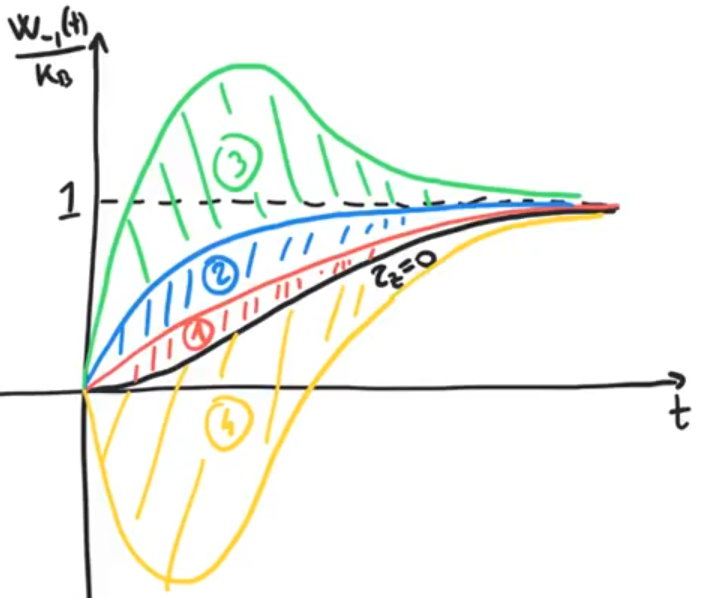
\includegraphics[width=\picwid]{secondo_ordine_con_zero}
\end{figure}

\newpage
\section{Realizzazione}
La \textit{realizzazione} è il procedimento che tenta di ricostruire un sistema
ISU a partire dalla funzione di trasferimento.

Si ricorda che per ogni sistema fisico esistono infinite ISU equivalenti,
mentre esiste una sola funzione di trasferimento, un'unica risposta all'impulso.
$$
(A,B,C,D) \longrightarrow W(s)
$$
La funzione di trasferimento è sempre esprimibile come un rapporto tra polinomi
$$
W(s) = \frac{b_ns^n+\ldots + b_0}
{s^n + a_{n-1}s^{n-1} + \ldots + a_0}
$$
Se $b_n=0$ il sistema diventerebbe strettamente proprio.
Sono in generale presenti $n+1$ coefficienti al numeratore ed $n$ al
denominatore, ossia $2n+1$ coefficienti totali.

Nell'ipotesi semplificativa di sistema SISO, alla rappresentazione ISU sono
associati i seguenti parametri
$$\begin{array}{*4c}
 (A & B & C & D) \\
 \uparrow  &\uparrow & \uparrow & \uparrow \\
 n^2 & n & n & 1
\end{array}$$
In totale saranno $n^2 + 2n + 1$, si vuole capire come ricostruire la ISU a
partire dalla funzione di trasferimento.

Tra le infinite soluzioni possibili sono presenti le cosiddette \textbf{forme
canoniche}, particolari strutture ISU composte da matrici con solo zeri o uno o
coefficienti con un numero massimo pari a $2n+1$.

\subsubsection{Forma canonica di raggiungibilità}

Si supponga di partire con una funzione di trasferimento in forma polinomiale,
si deve porre nella somma di una costante più un rapporto di polinomi eseguendo
una divisione.
$$
W(s) = \frac{\hat{b}_{n-1}s^{n-1} + \ldots + \hat{b}_0}
{s^n +a_{n-1} + \ldots + a_0}
+ \hat{b}_n$$
Va sempre normalizzato il denominatore e si ha $\hat{b}_n = b_n$ mentre il
generico coefficiente
$$
\hat{b}_i = b_i - a_ib_n, \qquad i=0,\ldots,n-1
$$
Le matrici del sistema possono essere scritti nel seguente modo:

$$
\begin{aligned}
A_R &= \begin{bmatrix}
0 & 1 & \dots & 0\\
0 & 0 & 1 & \dots & \\
\vdots & \vdots & \vdots & \vdots \\
0 & 0 & \dots  & 1 \\
-a_0 & -a_1 & \dots & -a_1
\end{bmatrix}
 &
B_R &= \begin{bmatrix}
0 \\ 0 \\ \vdots\\ 0\\ 1
\end{bmatrix}\\
C_R & = \begin{bmatrix}
\hat{b}_0 & \qquad &  \hat{b}_1& &\dots& & \hat{b}_{n-1}
\end{bmatrix} &
D_R&= \hat{b}_n = b_n
\end{aligned}$$


\subsubsection{Forma canonica di osservabilità}
Simile alle precedenti, i coefficienti del denominatore si trovano questa volta
nell'ultima colonna
$$\begin{aligned}
A_O &= \begin{bmatrix}
0 & \dots & 0 & -a_0\\
1 & 0 & \dots & -a_1\\
0 & 1 & \dots & \vdots\\
0 & 0 & 1 & -a_{n-1}
\end{bmatrix}&
B_O &= \begin{bmatrix}
\hat{b}_0 \\ \hat{b}_1 \\ \vdots \\ \hat{b}_{n-1}
\end{bmatrix}\\
C_O & = \begin{bmatrix}
0 & \dots & & 0 & & 1
\end{bmatrix} &
D_O &= \hat{b}_n = b_n
\end{aligned}$$

\subsubsection{Proprietà di dualità}
Le due forme canoniche sono l'una la duale dell'altra, è facile osservare che
$$
A_R = A_O^T,\qquad B_R = C_O^T,\qquad C_R=B_O^T,\qquad D_R=D_O
$$
C'è uno scambio di matrici tra ingresso e uscita, ottenuta una rappresentazione
si può sempre ricavare l'altra.
Sono presenti solo $2n+1$ parametri, dunque la scrittura delle matrici è
immediata.

\newpage
\section{Riassunto delle forme di rappresentazione dei sistemi}
\begin{itemize}
\item Equazione differenziale generale, lega le $y$ e le sue derivate alle $u$
e le sue derivate, una rappresentazione di tipo ingresso-uscita
\item ISU, utilizzando le regole di Cauchy si ottengono le quattro matrici
$A,B,C,D$
\item La funzione di trasferimento $W(s)$, a partire dalla ISU con la formula
$$
W(s) = C(sI-A)^{-1}B + D
$$
o viceversa mediante la \textit{realizzazione}.

Si ottiene a partire dall'equazione differenziale mediante il rapporto della
trasformata di Laplace dell'uscita e dell'ingresso, ricordando che la derivata
nel tempo corrisponde a moltiplicare per $s$.
Analogamente il processo inverso è simile.

\item Risposta all'impulso mediante la matrice $W(t)$, si ottiene
antitrasformando la funzione di trasferimento e viceversa.
Si ottiene a partire dalla rappresentazione ISU con la seguente
$$
W(t) = Ce^{At}B +D\delta(t)
$$
\end{itemize}

%\newpage
Si rappresenta di seguito uno schema riassuntivo delle varie tipologie di
rappresentazione e le diverse procedure di conversione
\begin{figure}[h]
\centering
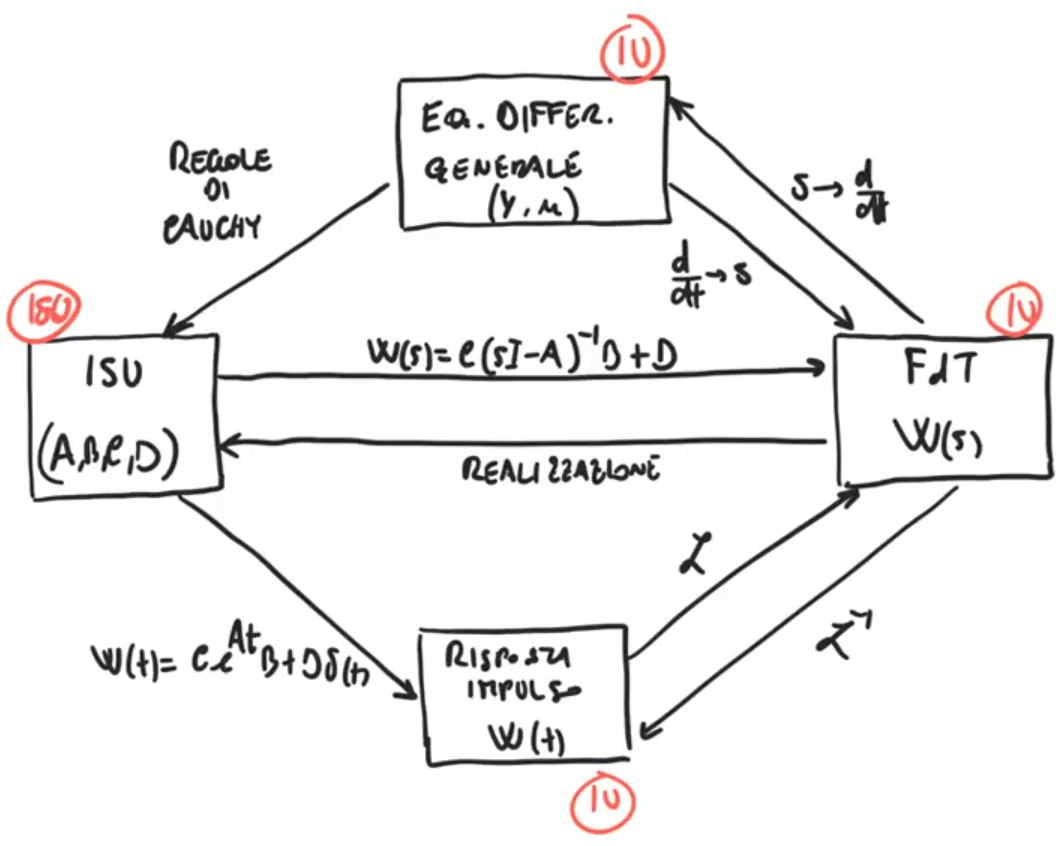
\includegraphics[width=0.75\linewidth]{schema_riassuntivo_sistemi}
\end{figure}


\chapter{Analisi in regime permanente}
Si supponga che il sistema sia asintoticamente stabile e ad esso si applica un
ingresso che non svanisce nel tempo, si avrà un'evoluzione iniziale ma
trascorso un certo tempo si avrà una risposta simile all'ingresso.
Si vuole determinare sotto quali ipotesi questa condizione è verificata.

\newpage
\textbf{Definizione di risposta in regime permanente}
$$
\forall \varepsilon>0 ,\ \forall x(t_0),\
\exists T_a\left(x(t_0)\right): t>T_a\left(x(t_0)\right)
\Rightarrow |y(t)-y_r(t)| < \varepsilon
$$
Con $T_a$ il tempo di attesa eventualmente funzione dello stato iniziale, $y_r$
la funzione analitica della risposta a regime.

Si supponga che esista la funzione $y_r(t)$, deve essere
indipendente dallo stato iniziale, nell'ipotesi di sistema lineare, usando le
formule di Lagrange
$$
y(t) = Ce^{A(t-t_0)}x(t_0)+\int_{t_0}^t
W(t-\tau)u(\tau)d\tau
$$
se si eseguisse il limite per $t\to \infty$ non si avrebbe più una funzione del
tempo, dunque nell'ipotesi che il sistema sia tempo invariante
si fa tendere l'istante iniziale $t_0$ in cui viene applicato l'ingresso a
$-\infty$, è analogo considerare un tempo all'infinito o un istante iniziale a
$-\infty$ ma in questo modo non si perde la variabile tempo nel risultato del
limite:
$$
y_r(t) = \lim_{t_0\to-\infty} \left(Ce^{A(t-t_0)}x(t_0)+\int_{t_0}^t
W(t-\tau)u(\tau)d\tau\right)
$$
La dipendenza da $x_0$ è solo presente nella componente libera, per $t_0\to
-\infty$ il coefficiente della matrice esponenziale tende a $+\infty$, se tutti
i modi del sistema hanno autovalore negativo, dunque il sistema è
asintoticamente stabile allora anche l'esponenziale tenderà a zero.

Se l'ingresso $u$ è una funzione regolare nel tempo ($W$ è sottinteso dato che
è composta da sole funzioni esponenziali)
$$
y_r(t) = \lim_{t_0\to -\infty} \int_{t_0}^t W(t-\tau) u(\tau)d\tau
\stackrel{t-\tau = \xi}{=} \int_{+\infty}^{0}W(\xi)u(t-\xi)(-d\xi) =
\int_0^{+\infty} W(\xi)u(t-\xi)d\xi
$$
Se l'integrale esiste finito, sarà sicuramente una funzione del tempo allora il
sistema ammette un regime permanete.
